Teaching machines to communicate about the visual world, ideally in natural language, is a long-standing topic of research, experiencing fascinating progress especially with the rise of deep neural network models \parencite{lecun2015deep, lake2017building}. 
One operationalization of this task that has received significant attention in computer vision is \textit{image captioning}, whereby models are trained to produce natural language descriptions of images, given example image-caption pairs. Importantly, the annotated data used for the training (e.g., datasets like MS COCO, \cite{chen2015microsoft}) is usually gathered by presenting the images to human annotators, asking them to produce true, possibly detailed, descriptions of the images. Therefore, such data can be rather considered \textit{descriptive}, but not optimized for a specific task.\footnote{Describing a picture can definitely be considered a communicative task. However, the notion of a specific task here is intended to delineate communication which is functional in the sense that it is intended to cause the recipient of the message to do something, i.e., act in the world \parencite{clark1996using, wittgenstein2010philosophical}. In this sense, captions produced by telling participants to just describe a picture, without embedding the message in an interactive setting, is non-functional.} Arguably, the training of such systems focuses on learning structural statistical patterns of how image pixels co-occur with certain text forms.

However, human language is fundamentally \textit{functional} in that we usually use it in order to communicate with other interlocutors, and do so in an somehow \textit{goal-directed} way---so as to make things happen in the world \parencite[e.g., ][]{wittgenstein2010philosophical, clark1996using}.\footnote{For simplicity, it is assumed that interlocutors are generally cooperative \parencite{grice1975logic}.} 
Research on modeling goal-directed communication has received increasing attention in the area of multi-agent communication. Here, functional aspects of communication are usually introduced by modeling two or more agents who use communication in order to complete a task \parencite{lazaridou2020multi}. This is typically modeled in the \textit{reinforcement learning} framework. This thesis focuses on functional---discriminative---communication about images and, therefore, is embedded in the multi-agent communication domain. 

This chapter reviews selected technical aspects and related work relevant to the main experiments of the thesis. Technical advances in machine learning architectures allowing to achieve state-of-the-art image captioning performance are reviewed in Section \ref{image_captioning}. The basics of reinforcement learning relevant for multi-agent communication are introduced in Section \ref{rl}. Table \ref{tab:defs} summarizes terms and abbreviations central for the remaining thesis. 

%Literature review notes go here. \pt{This more technical stuff should go into a chapter before multi-agent communication. It can be framed as background and approaches to image captioning which are traditional in the sense that they are supervised. The transition to multi-agent communication could be task-specific or -conditional communication about visual environment which is a critically functional part of human communication. Chapter AFTER multi-agents should be language drift (jacob, lewis, andreas, 2021: multitasking inhibits drift ).}

\begin{table}[]
	\centering
	%\begin{adjustbox}{width=1\textwidth}
	\begin{tabularx}{\textwidth}{|X|X|}
		\hline
		\textbf{Abbreviation / Term} & \textbf{Meaning / Definition}                                                                                                                          \\ \hline
		NN                           & Neural network                                                                                                                                         \\ \hline
		CNN                          & Convolutional neural network                                                                                                                           \\ \hline
		RNN                          & Recurrent neural network                                                                                                                               \\ \hline
		LSTM                         & Long short-term memory cell / layer, a type of RNN architecture proposed by \cite{hochreiter1997long}                                                                                                                         \\ \hline
		RL                           & Reinforcement learning                                                                                                                                 \\ \hline
		LM 						& Language model \parencite{jurafsky2000speech} \\ \hline
		Image vectors / features / embeddings & Vectorized numerical representations of raw images, usually produced by taking the output of the last layer of a trained CNN \\ \hline
		Speaker / sender             & Agent generating messages in a multi-agent communication reference game setting                                                                        \\ \hline
		Listener / receiver          & Agent receiving messages along with visual input and making the selection of the target referent in a multi-agent communication reference game setting \\ \hline
		
	\end{tabularx}
%\end{adjustbox}
\caption{\label{tab:defs}A table of abbreviations and commonly used terms the knowledge of which is presupposed for the reader. Please refer to, e.g., \cite{goodfellow2016deep} for an introduction.}

\end{table}


\section{Image Captioning}
\label{image_captioning}
Producing sensible and informative captions for images is a task that has received a lot of attention in machine learning research over the last years, developing from the more computer vision-centric task of object detection and recognition. %Specifically, image captioning in the supervised learning domain is facilitated by the availability of large-scale image-caption datasets like ``Microsoft Common Objects in COntext'' (MS COCO) \parencite{lin2014microsoft, chen2015microsoft}. %Importantly, in this domain, producing image captions in general is the only task of the developed applications; that. is, the captions are not supposed to target any particular actionable goal other than producing captions close to the human examples seen during training---they are \textit{task-unconditional}. \pt{Point is clear, but sharpen the actual formulation. } 
%From a machine learning perspective, the prerequisite for making image captions task-conditional would be the availability of supervised data from such a task. \pt{As discussed in the introduction, this motivates the choice of the multi-agent framework. Include and sharpen.} Nonetheless, technical advances developed in this domain provide the basis for agents employed in multi-agent settings; therefore, this section reviews selected work on image captioning in the computer vision and machine learning domain. 
This section focuses on introducing more recent \textit{deep} models for image captioning that can be applied to MS COCO because this dataset is used in presented work \parencite{lecun2015deep}; for an example of earlier work, see, e.g., \cite{kulkarni2013babytalk}.

One of the first end-to-end deep neural image captioning architectures was developed by \cite{vinyals2015show}. Their image captioner used a CNN-based image feature extractor in order to extract vector representations from raw images, which were fed into an LSTM-based recurrent \textit{decoder} module, trained end-to-end to maximize the likelihood 
\begin{equation}
\theta^* = \operatorname*{argmin}_\theta \sum_{(I, S)} log\; p(S \mid I; \theta) 
\end{equation}
of example image descriptions $S$, given the image vector $I$ and the network parameters $\theta$. The descriptions were vectorized by a trainable embedding layer through which they were passed before being passed through the LSTM. Figure \ref{fig:lstm} exemplifies the proposed training pipeline and the LSTM cell architecture. The hidden size of their LSTM was 512, and it was trained using the so-called teacher forcing mode (see Section \ref{model_pretraining} below for details). The minimized loss was the sum of negative log likelihoods of the target words at each time step (i. e., the cross-entropy loss). Only the last layer of the CNN which was initialized with weights from a model pretrained on ImageNet was trainable. Furthermore, dropout layers and ensebling of the model (i.e., combining predictions from several models) were used to produce the reported results. The authors used beam search as the decoding strategy during inference (see Section\ref{model_pretraining} for details) and achieved a BLEU-4 score of 0.272 on the MS COCO test set (see Section \ref{image_cap_metrics} below for details on evaluation metrics), next to comparably high results on other datasets. 
This architecture is closely related to the architecture of the sender agent in the present experiments. \cite{donahue2015long} also propose a very similar approach.

\begin{figure}
	\centering
	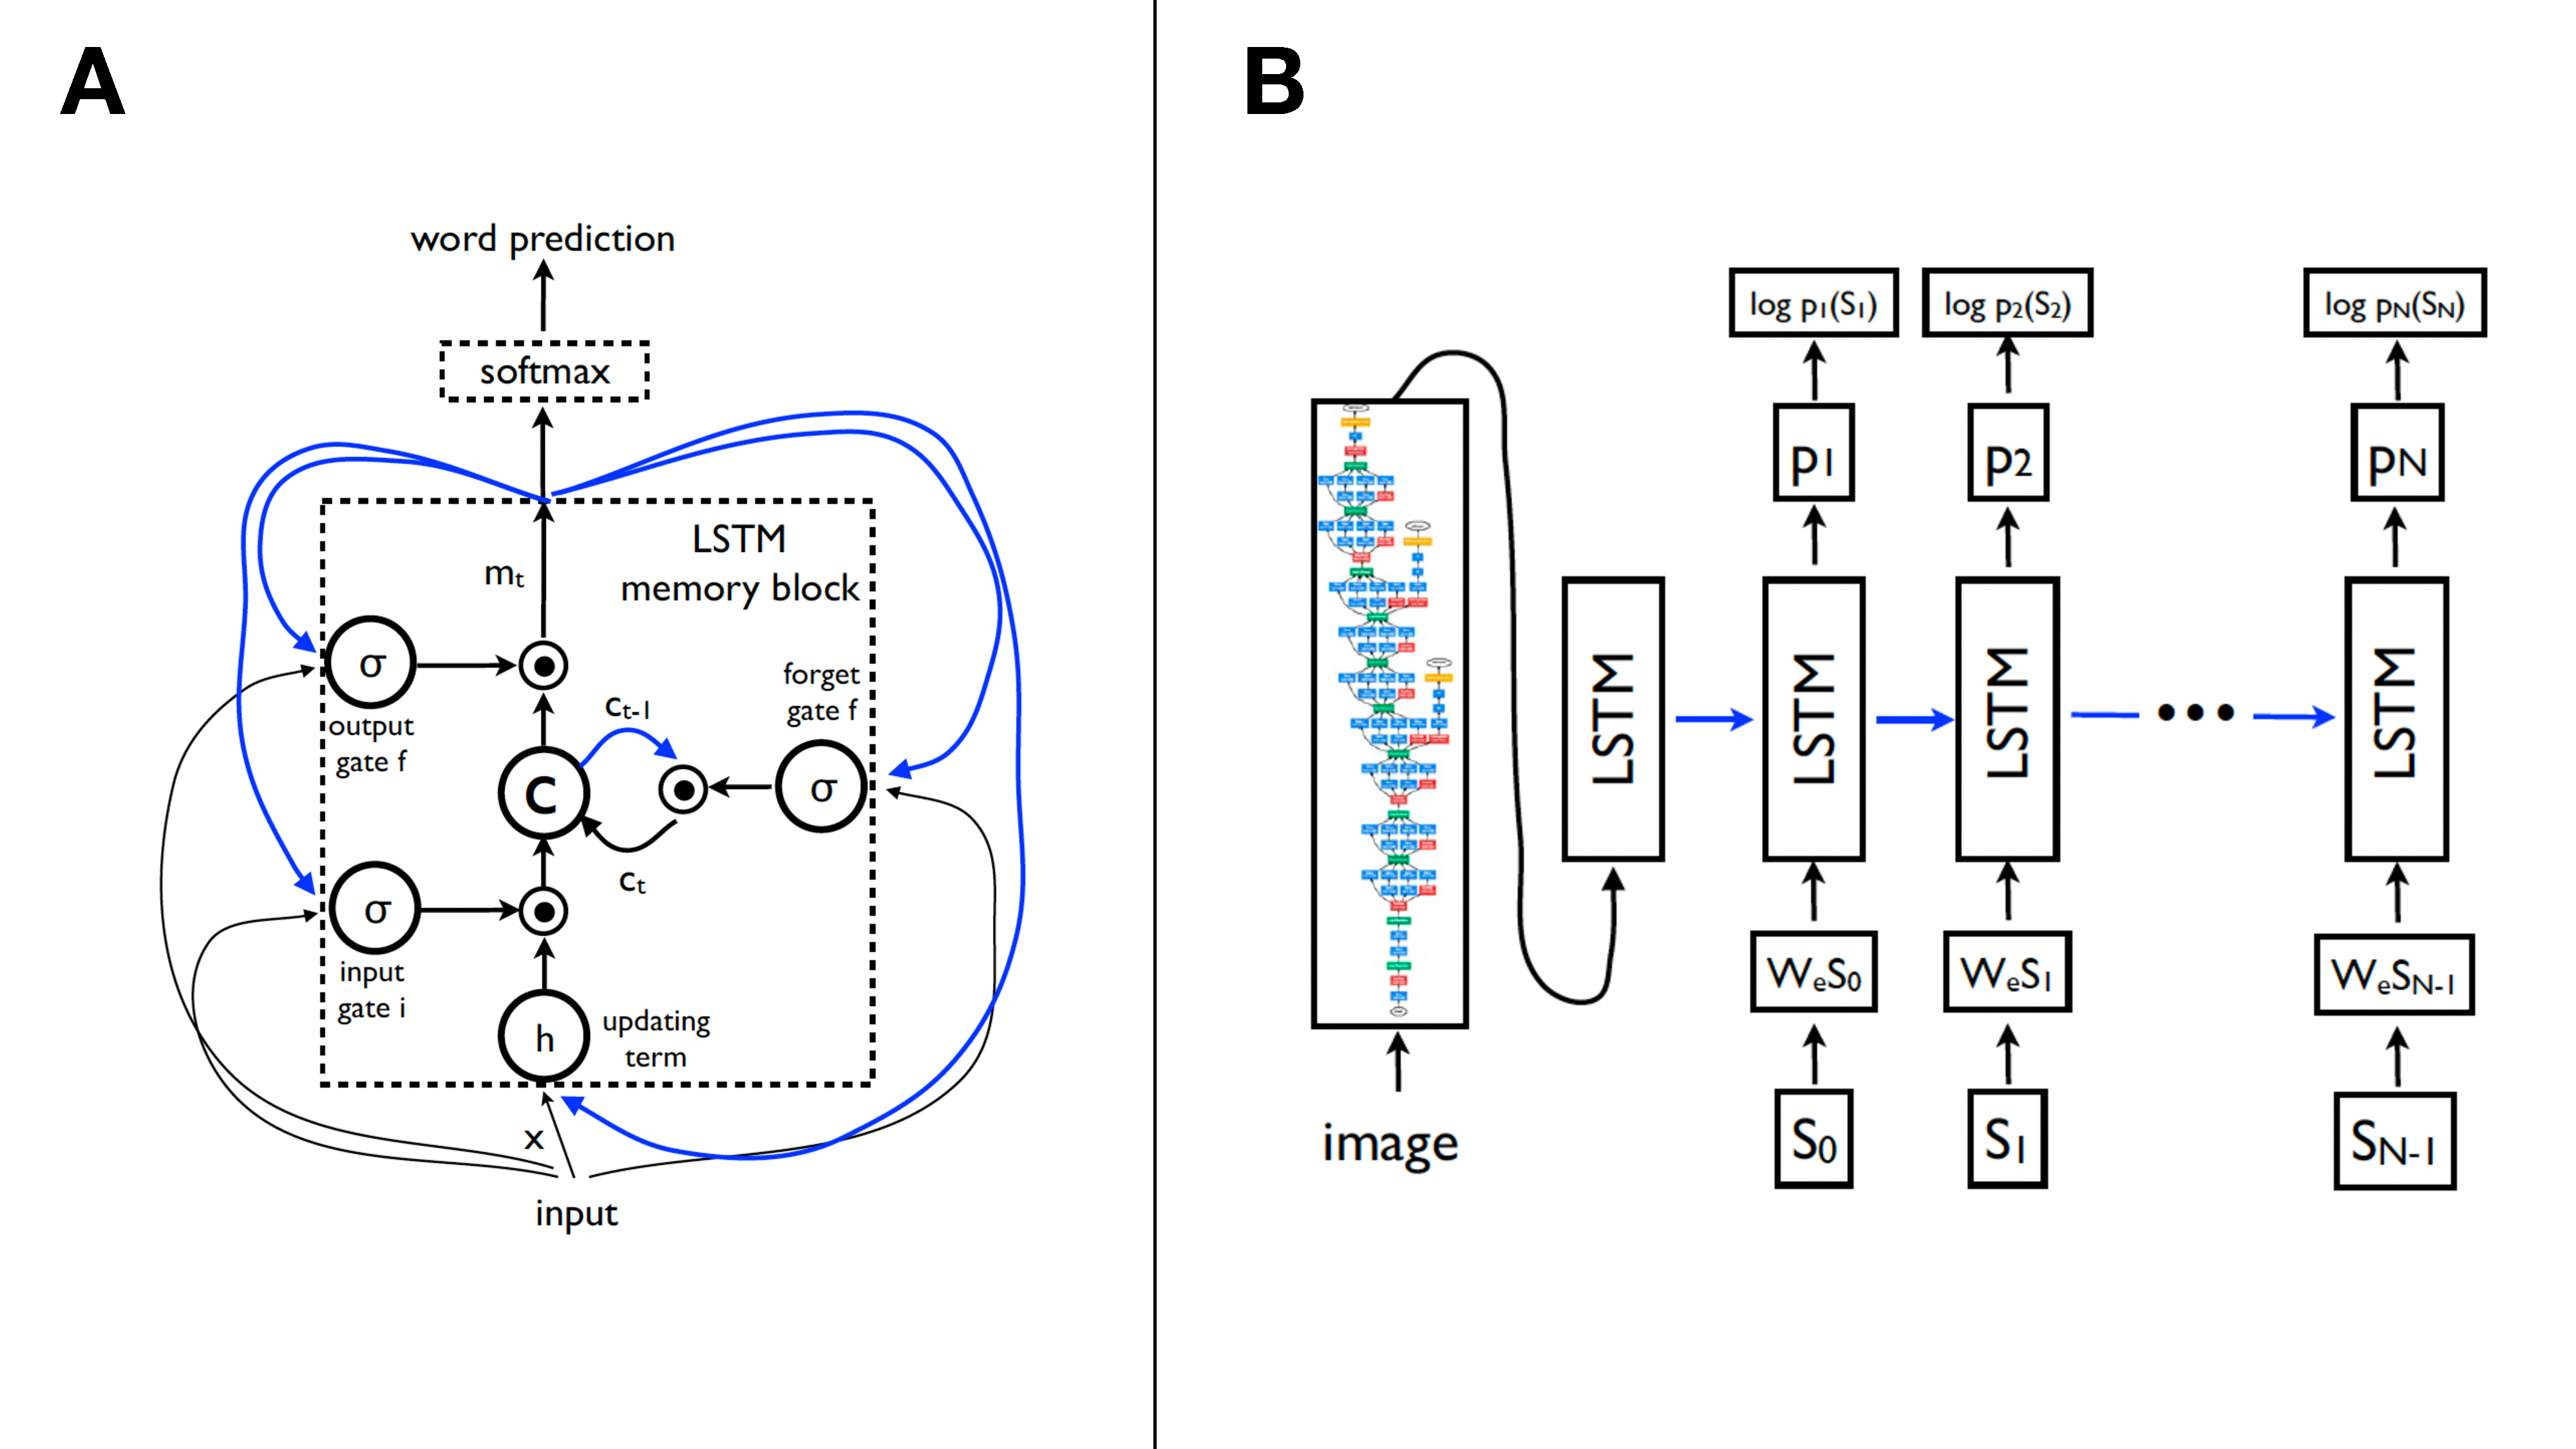
\includegraphics[width=\linewidth]{images/vinyals_lstm.pdf}
	\caption{A: LSTM cell architecture. B: Image captioner architecture consisting of a CNN image vector extractor (leftmost box) which passes an image vector into an LSTM cell (represented unrolled in time) as initialization of its hidden state \parencite[][p. 2--3]{vinyals2015show}.}
	\label{fig:lstm}
\end{figure}

Another system was developed by \cite{karpathy2015deep}; the main idea of their architecture was to align parts of images with relevant parts of the respective captions. 
Their first system consisted of a CNN pretrained on ImageNet which produces image embeddings, and a bidirectional RNN (BRNN) which produced embeddings of the corresponding captions in the same embedding space. Crucially, the BRNN was trained with a novel objective optimizing the alignment between ground truth captions and images via maximizing their dot product, while minimizing the dot product between images and incorrect captions. Using an additional  latent alignment variable the alignments produces sets of image regions annotated with (multi-word) phrases.
The learned alignments or full image-caption pairs were used as input data for a second image captioning model which consisted of a multi-modal RNN. It was trained to generate image captions with a mechanism akin to the one by \cite{vinyals2015show}, but adding the image vector at the first time step of the sequence only. \cite{karpathy2015deep} conducted experiments on different datasets including MS COCO. Ranking experiments evaluating the first model showed intuitively plausible image-phrase alignments, next to improved results compared to then state-of-the-art models. 
For evaluating the second model on full image captions, VGGNet image vectors were used, producing captions of decent quality as judged by standard evaluation metrics (see Table \ref{tab_coco_metrics_ref}). The model trained on region-phrase alignments was evaluated using human object annotations and was more consistent with those annotations than the full image model, indicating that the learned alignments were grounded correctly. In sum, their work is an interesting step towards generating captions based on more structured visual input.

\cite{xu2015show} propose a system where the image features are extracted using \textit{attention}, computed from annotation vectors representing parts of the image \parencite{bahdanau2014neural}. They compared stochastic attention to deterministic attention. The former was equivalent to the REINFORCE learning rule whereby the reward for the attention was proportional to the log likelihood of the target sentence (see Section \ref{rl_methods}). The latter was computed as a soft attention weight for the annotation vectors. This attention mechanism is diferentiable and, therefore, trainable end-to-end with back-propagation. The image location representation vectors were extracted using the VGGNet. For the experiment on MS COCO, they used a vocabulary size of 10,000. The soft attention architecture allowed to improve the test METEOR score on MS COCO by 0.02, while the hard attention did not yield an improvement, compared to \cite{vinyals2015show} (see Table \ref{tab_coco_metrics_ref}).

While the hitherto described systems consist of separate components used for representing the image and language parts, respectively, a different stream of work proposes \textit{joint multimodal} representations of images and captions. \cite{kiros2014unifying} learned a joint image-caption embedding space, using LSTMs for encoding the captions. Image representations extracted via a CNN were projected into the LSTM hidden states to create multimodal embeddings. The multimodal embeddings were trained by maximizing cosine similarity between the image embedding and LSTM hidden state for the target image-caption pair, while minimizing the similarity to distractors. These multimodal embeddings were passed to a decoder module of various architectures which was then tested on image-sentence ranking and image captioning tasks. They showed that multimodal embeddings outperformed object-detection based models.

Guided by the idea of creating combined representations, the most recent architectural innovation in this domain applies transformer layers for creating unified vision-language representations, ommiting the use of separate CNNs and RNNs \parencite{vaswani2017attention, zhou2019unified}. This work is motivated by advances achieved with pretrained language models, especially the BERT architecture \parencite{devlin2018bert}. The introduction of visual components in pretrained language model architectures is also called \textit{vision-language pretraining} (VLP). Typically, such models are built by first pretraining them on image-caption pairs on a masking task---i. e., predicting masked image patches or words---and then fine-tuning them on a downstream task \parencite[e.~g.,][]{lu2019vilbert}.
However, VLP architectures are usually developed either for image understanding like visual question answering or image classification, or generation tasks like image captioning \parencite{zhou2019unified}. 
\cite{zhou2019unified} proposed a unified model which can be used for both understanding and generation tasks. 
The model consisted of multiple transformer layers combining image and word embeddings and applying self-attention. It was pretrained on two objectives: reconstruction of masked caption tokens and sequence-to-sequence modeling. Such pretraining was shown to be comparable to other VLP architectures and to outperform other non-unified architectures on downstream tasks like MS COCO image captioning (see Table \ref{tab_coco_metrics_ref}). 

The experiments in this thesis closely follow the archtecture by \cite{vinyals2015show}. However, introduction of multimodal representation based models and more advanced networks as agents in multi-agent communication settings relying on visual input is an interesting direction for future work. 

\subsection{Model Pretraining}
\label{model_pretraining}
In this section, different approaches for training recurrent models which are predicting sequences, like the image captioning model is predicting a caption given the image, are discussed. In the context of multi-agent reference game experiments discussed in this thesis, this step can be seen as speaker agent pretraining.

It is assumed that the target task for the model is predicting the next token of a sequence, given the preceding tokens; this task is at the core of various applications like neural machine translation, image caption generation, text sumamrization and others \parencite[e.~g.,][]{cho2014learning, sutskever2014sequence}. Such tasks are usually modeled with recurrent neural networks \parencite{rumelhart1986learning}. The challenge when training recurrent neural network models which are predicting sequences at inference time by replicating this mode during train time, i.e., by conditioning the next token on the output of the model itself from the previous timestep during training, is slow convergence of the training, its instability and potentially poor generation skills \parencite{lamb2016professor}. The main training approach that has been proposed in order to mitigate these issues is \textit{teacher forcing} training, with several extensions to it: \textit{search over candidate output sequences}, \textit{curriculum learning} and \textit{professor forcing} \parencite{goodfellow2016deep, williams1989algorithm}.

When using curriculum learning, at each step the source of input to the next time step, i.e., whether it is the ground truth or the output of the previous timestep, is chosen randomly \parencite{bengio2015scheduled}. This curriculum anneals over time, starting at teacher forced learning only (i.e., all inputs are ground truth tokens) and gradually transitioning to using predicted inputs (so-called \textit{auto-regression}). Among several decay schedules for the probability of the next input token coming from the ground truth proposed by \cite{bengio2015scheduled}, inverse sigmoid decay schedule  was shown to yield best results on the MS COCO image captioning task.

When using professor forcing, the discrepancy between the training and inference performance is addressed by minimizing the discrepancy between the teacher forced and auto-regressive sampling behaviour, i.e., by making the distribution over sequences during training maximally similar to the target distribution \parencite{lamb2016professor}. This is achieved by training the model as a Generative Adversarial Network (GAN). More specifically, a second recurrent network---a biderectional RNN---  is introduced additionally to the RNN generating the captions. Due to the additional overhead for training an image captioner with this approach, exploring the effects of such pretraining on downstream multi-agent communication tasks is left for future work.

An additional important aspect of using recurrent networks for inference is the strategy used to pick a single predicted token at each timestep (i.e., the \textit{decoding strategy}). A standard approach is the \textit{greedy} decoding wherein the token with the highest probability is selected at each timestep. Alternatively, search over output sequences, or, \textit{beam search} decoding maintains a beam of $k$ best alternatives and selects a sequence with the highest probability. This work uses the term \textit{pure} decoding (or, sampling) in reference to a strategy wherein the token is selected via sampling from the categorical distribution over the vocabulary produced by the recurrent network at each timestep. Other strategies also exist. 

For conducting the experiments in this thesis, speakers pretrained with different following approaches were considered during initial exploratory grid searches: pure teacher forcing pretraining, constant 0.5 rate teacher forcing, adaptive teacher forcing rate pretraining (decreasing the rate by the factor 0.5 in each training epoch), scheduled sampling and top-$k$ sampling with temperature 2 (replicating \cite{lazaridou2020multi}). Details of the grid search are presented in Appendix \ref{app:grid_search}. The speakers used in reported experiments were pretrained using the adaptive teacher forcing rate and pure decoding. If not stated otherwise, pure decoding was used in the reported experiments. \pt{Greedy experiments will be added if time allows.}

\subsection{Evaluation Metrics}
\label{image_cap_metrics}

\begin{figure}
	\centering
	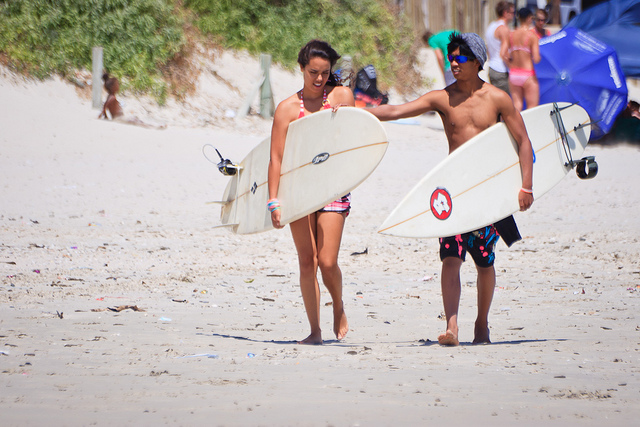
\includegraphics[width=0.7\linewidth]{images/COCO_train2014_example.jpg}
	\caption{Example image from the MS COCO Captions train split \parencite{chen2015microsoft}. The corresponding captions provided by human annotators are: ``The two people are walking down the beach.'', ``Two people carrying surf boards on a beach.'', ``Two teenagers at a white sanded beach with surfboards.'', ``A couple at the beach walking with their surf boards.'', ``A guy and a girl are walking on the beach holding surfboards.''. }
	\label{fig:coco_example}
\end{figure}

Another important yet non-trivial aspect of developing image captioning systems is their evaluation. Image captioning has been considered difficult to evaluate because for a given input image, several output captions might be equally suitable (e.~g., see Fig. \ref{fig:coco_example}). Therefore, usually a suite of evaluation metrics is used. This work employs the metrics proposed for the MS COCO dataset \parencite{chen2015microsoft}: BLEU-$n$ ($n$ denoting the length of used $n$-grams), METEOR and CIDEr scores. In this section, conceptual aspects of these metrics applied to image captioning are introduced; for formal derivations, see, e. g., \cite{chen2015microsoft}.\footnote{The implementation of these metrics in Python provided by \url{https://github.com/daqingliu/coco-caption} is used in the present experiments.}

The BLEU-$n$ score evaluates the co-occurence on $n$-grams between generated and reference sequences \parencite{papineni2002bleu}. More precisely, the corpus-level $n$-gram precision is computed (fraction of ground truth $n$-grams in the generated $n$-grams). That is, all reference captions are considered as a corpus, and the overall score is computed as a weighted geometric mean over all $n$-grams. However, BLEU favors short sentences and has been shown to be a poor metric for single sentence comparisons, especially when considering longer $n$-grams.

%The ROUGE metric was developed for text summarization evaluation and has three variations: ROUGE$_N$, ROUGE$_L$ and ROUGE$_S$. ROUGE$_N$ computes $n$-gram recall over all ground truth captions given the generated one (=fraction of found ground truth n-grams); ROUGE$_L$ is the $F$-score computed over the lengths of so-called \textit{Longest Common Subsequence} (i.e., an n-gram where other words may occur in between). Finally, ROUGE$_S$ is computed as $F$-score over counts of skip bigrams (i.e., bigrams where k words may occur in between).  Generally, the ROUGE scores are somewhat better at capture longer-range sentence structure preservation.

METEOR is computed by generating alignments between target and generated captions \parencite{banerjee2005meteor}. The alignments are based on both matching exact tokens and matching WordNet synonyms, stems and other generalizations. Then, the harmonic mean between the precision and recall over the best target-generated caption pairs is computed, and the final score includes a penalty for quality of the found alignments. METEOR is computed as a corpus level metric, as well, meaning that all target captions are aggregated.
 
Finally, CIDEr is a native image captions evaluation metric \parencite{vedantam2015cider}. It is computed as a weighted TF-IDF for each $n$-gram occurring in the ground truth captions for the set of all images. Intuitively, the TF-IDF weighting provides a trade-off between common and distinctive $n$-grams. These weights are then combined into vectors for each $n$-gram of length $n$, based on which average cosine similarity between vectors for ground truth and generated captions is computed. The final CIDEr score is obtained as the average over the single n-gram similarities. In order to increase the similarity of metric results to human intuitions, further modifications including caption length-based gaussian penalties are included. Intuitively, CIDEr captures the similarity in distinctness or saliency of the generated and ground truth captions.

These metrics can only be computed in the presence of ground truth image captions. They are applied in both experiments on the MS COCO dataset and on the 3Dshapes dataset. Here, the self-generated captions are treated as ``ground truth'' (see Section \ref{ds:3dshapes}).
Previous work on captioning the MS COCO datase discussed in this section provides a baseline for evaluating the quality of captions produced in this work. Table \ref{tab_coco_metrics_ref} provides and overview of scores achieved with extant systems.

\begin{table}[]
	\begin{tabularx}{\textwidth}{|X|l|l|l|l|l|l|l|}
		\hline
		Model                               & BLEU-1 & BLEU-2 & BLEU-3 & BLEU-4 & METEOR & CIDEr \\ \hline
		\cite{bengio2015scheduled}        & -      & -      & -      & 0.323   & 0.254  & 0.987 \\ \hline
		\cite{vinyals2015show}  & -      & -      & -      & 0.277    & 0.237  & 0.855 \\ \hline
		\cite{xu2015show} & 0.718  & 0.504  & 0.357  & 0.250     & 0.239  & -     \\ \hline
		\cite{karpathy2015deep}          & 0.625  & 0.450  & 0.321  & 0.230   & 0.195  & 0.660 \\ \hline
		\cite{zhou2019unified}          & -  & -  & -  & 0.365   & 0.284  & 1.169 \pt{?} \\ \hline
	\end{tabularx}
\caption{\label{tab_coco_metrics_ref}The table shows evaluation metrics results for the quality of captions generated on respective test sets of the MS COCO dataset. Best results reported in each paper are included.}
\end{table}

\section{Reinforcement Learning}
\label{rl}

Given the foundations of image captioning architectures, this section provides the theoretical tools for embedding these architectures into goal-directed interactive frameworks like multi-agent communication.

\subsection{Introduction}
A natural choice for training interacting artificial agents to complete certain tasks like language games is reinforcement learning (RL), as ``[r]einforcement learning is a computational approach to understanding and automating goal-directed learning and decision-making'' \parencite[][p.~15]{sutton2018reinforcement}. Next to supervised and unsupervised learning, it represents one of three major paradigms in machine learning. 
%In this framework, the agents learn to make decisions as to which actions to take, given the environment, and receive responses to those actions from the environment putting the agents into new states . This repeats iteratively, until the agents learn how to effectively reach the desired goal state. For instance, the goal state can be understood as winning a game or successfully completing a communicative task. 
%``The reinforcement learning problem is meant to be a straightforward framing of the problem of learning from interaction to achieve a goal. The learner and decision-maker is called the agent. [...] These interact continually, the agent selecting actions and the environment responding to those actions and presenting new situations to the agent.'' (p.53). 
%A particular task is defined in terms of a complete definition of the environment, representing a particular instance of reinforcement learning (p. 54).

More precisely, reinforcement learning problems can be defined as learning the mapping from situations, represented as \textit{environments}, to optimal \textit{actions} that agents may choose in order to achieve task (sub-)goals, while maximizing the \textit{reward} signal \parencite{sutton2018reinforcement}. The reward can be understood as the environment's feedback about the optimality of the action with respect to achieving the goal (see Fig. \ref{fig:rl}). The chosen actions put the agent into new states. This repeats iteratively, until the agents reach the desired goal state or other interaction stopping conditions are met. For instance, the goal state can be understood as winning a game or successfully completing a communicative task. 

\begin{figure}
	\centering
	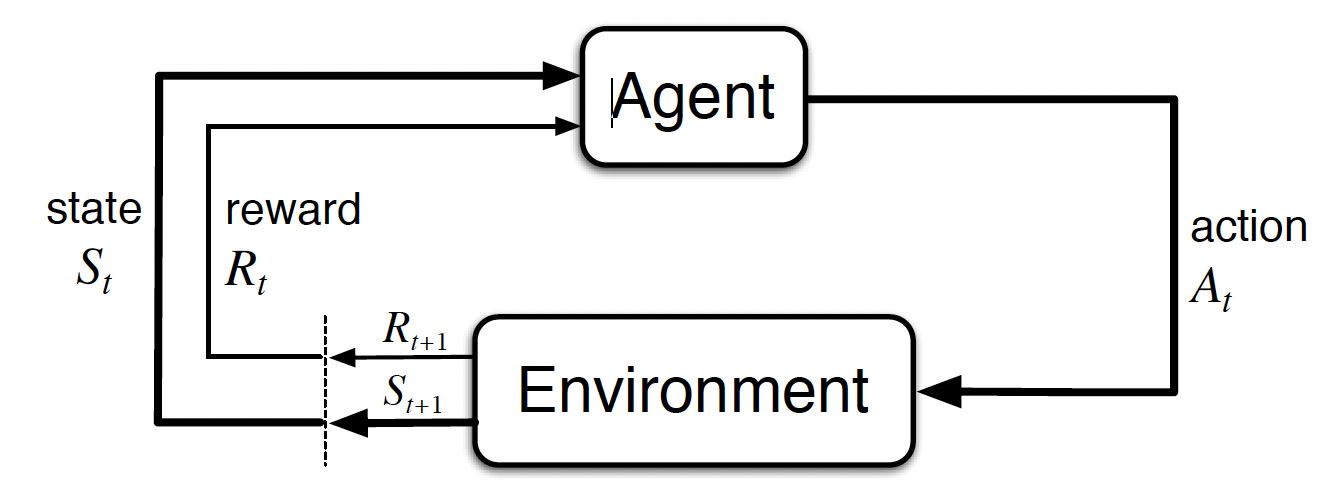
\includegraphics[width=0.8\linewidth]{images/rl_intro.png}
	\caption{Interaction of the environment with the agent via states, actions and rewards \parencite[][p. 48]{sutton2018reinforcement}.}
	\label{fig:rl}
\end{figure}

%The most important building blocks of RL systems are defined below: \pt{Definitions of: reward, environment, agents, actions, states, policy, value function, if necessary, q-learning maybe. An optiional model of the environment may also exist. }
% \begin{itemize}
%	\item agent: learner and decision maker in the interaction who tries to achieve a goal for a certain task.
%	\item environment: the setting in which the agent's interactions are situated, everything outside of the agent itself.
%	\item policy: the agent's learned mapping from environment states to actions within the environment. 
%	\item reward signal: \pt{TBD} numerical representation of the quality single \textit{rewards} the agent receives at each timestep of the decision process. Improtantly, the agents' goal is to maximize the sumn of the rewards over the task completion.
%	\item value function: a function mapping states to expected total reward for agents starting the actions at the given state. These are adapted and reestimated based on observed action and reward sequences of the agents over their lifetime. \pt{TBD}
%\end{itemize}

Decision making sequences modeled by reinforcement learning are standardly formalized as Markov Decision Processes (MDPs). 
It is assumed that the interaction takes place over discrete timesteps $t = 0,1,2 ...$.\footnote{Reinforement learning can also be applied to continuous state and action spaces. These aspects are ommitted in this introduction for brevity reasons.} At each step $t$, the state $S_t \in \mathcal{S}$ is the state the agent is currently in, where $\mathcal{S}$ is the set of all possible states. Given the state, the agent selects an action $A_t \in \mathcal{A}(s)$, where $\mathcal{A}(s)$ denotes the set of all actions available in state $S_t$ at timestep $t$. At the next timestep $t+1$, the agent receives a reward $R_{t+1} \in \mathcal{R}$ for the action $A_t$ in state $S_t$. These iterations can be formalized as \textit{finite} MDPs if they consist of an $\mathcal{A}, \mathcal{S}$ and $\mathcal{R}$ with finite numbers of elements. In this case, the probability $p$ for a particular state $s'$ and reward $r'$ to occur at time $t$, conditioned on the previous state and action, is well-defined \parencite[][p. 48]{sutton2018reinforcement}:  
\begin{equation}
p(s', r' \mid s, a) \doteq Pr(S_t = s', R_{t+1} = r' \mid S_{t-1} = s, A_{t-1} = a)
\end{equation}
Given $p$, one can then compute \textit{state transition probabilities} $\mathcal{T}$ (i.e., probabilities for reaching a particular state given previously visited states) 
\begin{equation}
p(s' \mid s, a) = \sum_{r \in \mathcal{R} } p(s', r \mid s, a)
\end{equation}
and, most critically, the expected rewards for given state and action combinations \parencite[][p. 49]{sutton2018reinforcement}: 
\begin{equation}
\E [R_t \mid S_{t-1}=s, A_{t-1}=a]
\end{equation}
The state transition probabilities and the function $p$, respectively, characterise the environment dynamics and, therefore, the MDP is modelled by the tuple $\langle \mathcal{A}, \mathcal{S}, \mathcal{T}, \mathcal{R} \rangle $. An assumption often made in the RL literature is that the states have the \textit{Markov property}, i.e., that they encode information from all previous interaction steps.

Expected rewards are especially important in order to estimate the \textit{return} $G$ and thus, formally represent the objective of learning---maximizing the return. In present work, the following simple definition of $G_t$ is assumed: 
\begin{equation}
G = R_{t+1} + R_{t+2} + ... + R_T
\end{equation}
where $T$ is the final step of the action sequence and $R_{t+1}$ represents the reward received for the action $A_t$. These interaction iterations yielding returns are also called \textit{episodes}. Different return formalizations, e. g., using expected \textit{discounted} rewards, are used in other applications for episodic tasks. However, a discount cannot really be applied in the presented reference game experiments since the environment only provides one reward per entire episode (i.e., entire message generation; see below for details).

The mapping from actions and states to rewards is specified by the \textit{value function}. Since collected reward values depend on the taken actions, the last critical component of RL environments is the policy. ``A policy is a mapping from states to probabilities'' of taking available actions: $\pi(a | s)$ describes the probability that the agents chooses the action $a$ in the state $s$. The central problem of RL is then the estimation of an optimal policy, i.e., one yielding the maximal return. The following section reviews different methods for estimating the policy, especially focusing on methods applicable to \textit{deep RL} \parencite{lecun2015deep}, i.e., RL with deep neural network agents akin to the ones used in presented experiments. The overview is provided on a conceptual level, only providing more details for the algorithm used in the presented work.

%The central problem of RL is the estimation which action to take at each step in any state in order to maximize the return. To this end, in \textit{value-based approaches} the value function is estimated, which describes how valuable it is with respect to the expected return for an agent to be in a given state. 
%Terminal state = state at the end of each episode.
% Concrete specification and notation of actions, rewards, states and policy.
%Value functions and optimal policies (up to p. 95).
%Transition to deep reinforcement learning \parencite{lecun2015deep}.
\subsection{Deep Reinforcement Learning Methods}
\label{rl_methods}
Two main types of RL algorithms are usually distinguished in the literature: \textit{value based} and \textit{policy gradient based} methods. 

The main idea behind \textbf{$Q$-learning methods} is the construction of an action-value function called $Q$, making $Q$-learning a value-based method \parencite{sutton2018reinforcement}. The function is learned independently of the corresponding policy, although the learning proceeds via iterating over the steps of an episode and selecting actions according to a policy derived from the current estimate of the action-value function. In deep Q-learning, the function $Q$ is represented by deep neural networks \parencite[e.g.,][]{hester2018deep}. For an overview of different policy derivation methods, see \cite{sutton2018reinforcement}. 

The so-called \textbf{Actor-Critic method} also belongs to the class of value based methods, although both a policy and a value function are learned \parencite{sutton2018reinforcement}. It consists of an actor learning a policy from which the actions are sampled, and a critic, which is estimating the action value function of the currently used policy. The goal hereby is to estimate whether the action chosen based on the current policy improves the return compared to its expected value. Based on the feedback from the critic, the policy is updated. 

In contrast, so-called \textbf{policy-gradient methods} focus on improving the parameters of the policy directly \parencite{sutton2018reinforcement, sutton1999policy, williams1992simple}. %More specifically, this approach provides a solution to the issue of computational intractability of analytically solving for an optimal policy (p. 80) and instead focuses on the agent's experience simulated from the environmant.  
More specifically, the policy is approximated stochastically with a parametrized function, e. g., a neural network. The policy is learned by optimizing the parameters $\theta$ of the model with respect to performance $\rho$ of the agent (e.~g., rewards) at each step \parencite[][p. 1058]{sutton1999policy}: 
\begin{equation}
\Delta \theta \approx \alpha \frac{\partial \rho}{\partial \theta} 
\end{equation}
The \textit{policy gradient theorem} proves that this performance based gradient can be estimated even though rewards depend on explicit knowledge of the environment. It provides the derivation of an analytic expression which does not depend on the unknown distribution of states dictated by the policy and yielding the rewards. See \cite[][p. 326f.,]{sutton2018reinforcement} for the formal derivation.

This introduction is constrained to a particular policy-gradient method---the algorithm REINFORCE---which is used in the presented experiments \parencite{williams1992simple}. For discussion of further policy-gradient methods, see, e.g., \cite{sutton2018reinforcement}. 
The REINFORCE algorithm posits that a locally optimal policy can be obtained by updating each weight $w_{ij}$ of the policy network accoring to 
\begin{equation}
\label{eq:reinforce}
\Delta w_{ij} = \alpha_{ij} (r - b_{ij}) \frac{\partial \; log(\pi)}{\partial \; w_{ij}}
\end{equation}
where $\alpha_{ij}$ is the learning rate, $r$ is the reward, $b_{ij}$ is the baseline (see below for details) and $\pi$ is the policy \parencite[cf.][p.~234]{williams1992simple}. The update depends on a gradient on the right-hand side; the policy gradient theorem shows that it is proportional to the expectation of a sample gradient. So when $r$ is available for each timestep including the last step of the episode, tractable weight updates can be computed retrospectively for the entire episode by applying \textit{Monte-Carlo} approximation. That is, the average over episode returns that are received based on observing an episode starting from an arbitrary policy and iteratively improving it are compute \parencite{sutton2018reinforcement}. Intuitively, the method selects weights proportionally to the expected return. One generally problematic aspect of Monte-Carlo methods is the behavior called \textit{exploitation} whereby actions that are selected more frequently are further sampled such that no information is learned about alternative actions. One way of maintaining sufficient \textit{exploration} (sampling new actions) is summarized below. 

Applied to sender agents in a multi-agent communication framework, the policy is the conditional probability distribution over message tokens, given previous tokens. The tokens are, therefore, the available actions. An episode is then the sampling of an entire message.\footnote{Alternatively, one can consider reference games as episodic tasks where each episode only consists of one timestep.} The reward is the signal based on the task success, received upon producing the message. The goal is to learn to select the tokens so as to achieve the goal of the communication task with maximal rewards. Since the number of different tokens the agent may choose from at each timestep may be large in real-world application \parencite[cf.][]{he2015deep}, learning such an optimal policy remains a computationally difficult task.

One solution potentially stabilizing the learning in REINFORCE-based algorithms is the \textbf{selection of the baseline} $b_{ij}$ (cf. Eq. \ref{eq:reinforce}), which has been shown to significantly reduce the variance in many algorithms \parencite{sutton2018reinforcement}. 
Among other possibilities, the baseline can be represented by the running mean over the rewards, by a learned state value function, or a constant, and different studies investigate its effects on convergence speed and task performance \parencite{williams1992simple, greensmith2004variance}. However, upon initial exploratory simulations the addition of a mean baseline did not yield observable improvements of presented experiments and is, therefore, omitted in all conducted experiments. 

Another method for achieving more stable convergence of the policy is \textbf{entropy regularization} \parencite{williams1991function, mnih2016asynchronous}. More specifically, this method encourages the \textit{exploration} behaviour of the agents by encouraging the selection of states with high entropy, by adding a weighted entropy term to the policy based weight updates introduced in Eq. \ref{eq:reinforce}: 
\begin{equation}
\Delta w_{ij} = \alpha_{ij} (r - b_{ij}) \frac{\partial log(\pi)}{\partial w_{ij}} + \beta (- \sum_{A_t \in \mathcal{A}(s)} \pi(A_t \mid S_t) \; log \; \pi(A_t \mid S_t))
\end{equation}
The disadvantage of using entropy regularization is the introduction of an entropy weight $\beta$ as an additional hyperparameter to be tuned. However, it has been successfully used in practice and is also included in presented experiments.

To sum up, this chapter reviewed related work on image captioning, which is the operationalization of the communicative task investigated in this thesis. Different model architectures as well as important practical training aspects were presented. Among those, special focus was put on models consisting of RNN-based language modules combined with CNN-based vision modules, paving the ground for presenting agent architectures in own experiments.  
Furthermore, important theoretical aspects of reinforcement learning were presented, allowing to better understand multi-agent communication experiments. 

The next chapter describes how the methods introduced in this chapter come together in practice in work on multi-agent communication.

%\pt{stationary distribution?}
%\pt{Add machine details in the expts section}